\documentclass[12pt]{article}
\usepackage{preamble}

\pagestyle{fancy}
\fancyhead[LO,LE]{Математический анализ}
\fancyhead[CO,CE]{28.02.2024}
\fancyhead[RO,RE]{Лекции Далевской О. П.}


\begin{document}
    Теорема: $\displaystyle J^\prime_\alpha = \left(\int^b_a f(x, \alpha)dx\right)^\prime_\alpha = \int^b_a f^\prime_\alpha(x, \alpha)dx)$

    Ex:

    $\displaystyle I(\alpha) = \int^{+\infty}_0 e^{-x} \frac{sin\alpha x}{x}dx$
    $\displaystyle I^\prime_\alpha(\alpha) = \int^{+\infty}_0 (e^{-x} \frac{sin\alpha x}{x})^\prime_\alpha dx = \int^{+\infty}_0 e^{-x} \frac{1}{x} x cos\alpha x dx =
    \int^{+\infty}_0 e^{-x} cos\alpha x dx = \frac{1}{a + \alpha^2}$

    Из этого следует, что $\displaystyle I(\alpha) = \int_{+\infty}_{0} \frac{1}{a + \alpha^2} dx = arctg(\alpha) + C$

    Так как $I(\alpha)$ - несобственный интеграл, это функция, а не семейство функций. Найдем $C$.

    $\displaystyle I(0) = \int^{+\infty}_0 e^{-x} \frac{sin 0 * x}{x}dx = 0 \Longrightarrow C = 0$
    Таким образом, $\displaystyle I(\alpha) = (\int^{+\infty}_0 e^{-x} \frac{sin\alpha x}{x} dx)^\prime_\alpha = arctg(\alpha)$

    Ex: Гамма-функция

    \[\Gamma(\alpha) = \int^{+\infty}_0 x^{\alpha - 1} e^{-x} dx \quad (\alpha > 0)\]

    Исследуем на сходимость:

    \[\Gamma(\alpha) = \int^{+\infty}_0 x^{\alpha - 1} e^{-x} dx = \int^{1}_0 x^{\alpha - 1} e^{-x} dx + \int^{+\infty}_1 x^{\alpha - 1} e^{-x}\]

    На отрезке $[0; 1]$ $e^(-x) \in [0;1]$.
    Тогда $\displaystyle 0 \leq \int^{1}_0 x^{\alpha - 1} e^{-x} dx \leq \int^{1}_0 x^{\alpha - 1} dx \Longrightarrow$ интеграл сходится

    Пусть $n > \alpha - 1, n \in \Natural$, тогда:

    $\displaystyle \int^{+\infty}_1 x^{\alpha - 1} e^{-x} dx \leq \int^{+\infty}_1 x^{n} e^{-x} dx$ - по частям, появятся $\dislpaystyle x^{k} e^{-x} \Big|^{+\infty}_1 \rightarrow 0$ и $\dislpaystyle \int^{+\infty}_1 e^{-x} dx$ сходится

    Найдем формулу для $\Gamma(\alpha)$:

    $\displaystyle \alpha \in \Natural \quad \Gamma(1) = \int^{+\infty}_0 e^{-x} dx = -e^{-x} \Big|^{+\infty}_{0} = 1$

    $\displaystyle \Gamma(\alpha) = \int^{+\infty}_0 x^{\alpha - 1} e^{-x} dx = -\int^{+\infty}_0 x^{\alpha - 1} de^{-x} = -x^{\alpha - 1}e^{-x} \Big|^{+\infty}_1 + \int^{+\infty}_0 x^{\alpha - 2} (\alpha - 1) e^{-x} dx = (\alpha - 1) \Gamma(\alpha - 1) = $
    $(\alpha - 1)! \Gamma(1) = (\alpha - 1)!$

    $\Gamma(n + 1) = n!$

    Lab: Посмотреть, как обобщается понятие факториала на вещественные числа:

    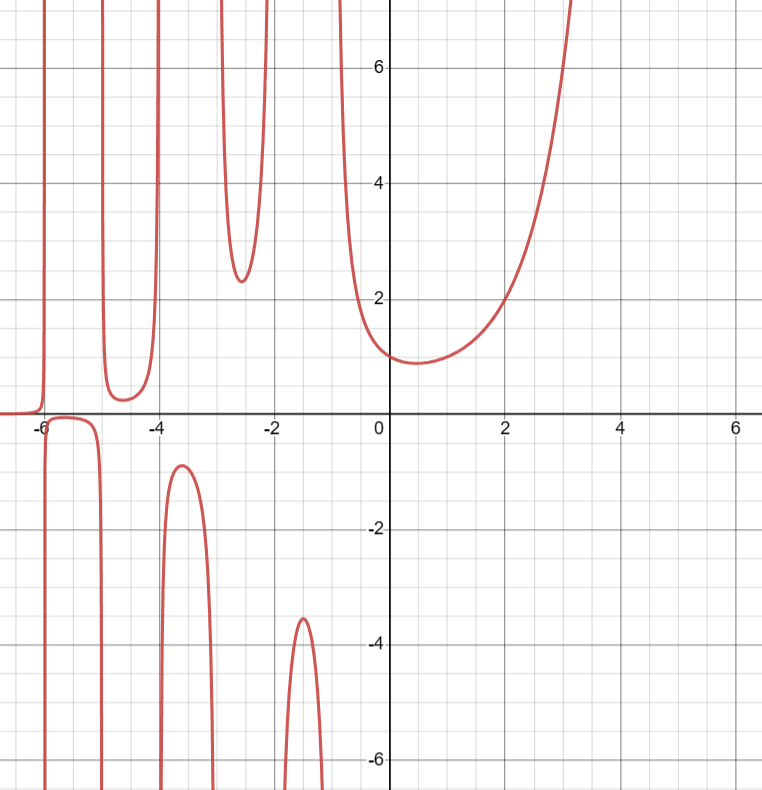
\includegraphics[height=70mm]{images/calculus_2024_02_28_1}

    \vspace{20mm}

    \textbf{4. Функция нескольких переменных (ФНП)}

    \textbf{4.1. Определение}

    \vspace{5mm}

    Nota: Дадим определение ФНП

    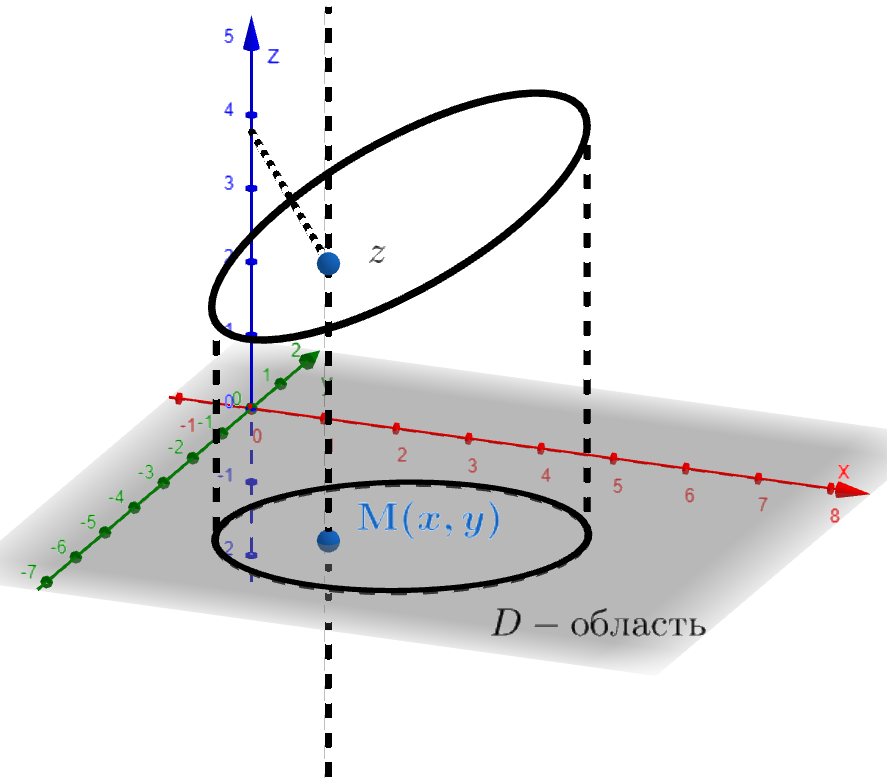
\includegraphics[height=90mm]{images/calculus_2024_02_28_2}

    $\forall M(x, y) \exists! z \in \Real : z = f(x, y) \Longleftrightarrow z = f(x, y)$ - функция двух переменных

    Def: Окрестность точки $M_0(x_0, y_0)$

    $U_\delta (M_0) = \Set{(x, y) \in Oxy : (x - x_0)^2 + (y - y_0)^2 < \delta^2, \delta > 0 \text{ - радиус}}$

    $\stackrel{o}{U}_\delta (M_0)$ - выколотая

    Nota: $\Delta x = x - x_0, \Delta y = y - y_0$, одновременное стремление $\Delta x, \Delta y \rightarrow 0$
    можно заменить $\Delta \pho = \sqrt{(x - x_0)^2 + (y - y_0)^2} \rightarrow 0$\\[1\baselineskip]


    Def: $\displaystyle \lim_{M \to M_0} z(x, y) = L \in \Real \Longleftrightarrow \forall \varepsilon > 0 \exists \delta > 0 (\delta = \delta(\varepsilon)) | \forall M \in \stackrel{o}{U}_\delta(M_0) \text{ } |z(x, y) - L| < \varepsilon$

    $M_0$ - точка сгущения и $x_0, y_0 \in \Real$ (здесь)

    Nota: На плоскости $Oxy$ возможно стремление $M \rightarrow M_0$ по разным путям $F(x, y) = 0$ (уравнение кривой)

    При этом значение предела вдоль разных путей могут отличаться (аналог односторонних пределов)

    Предел в определении - предел в общем смысле: его существование и значение не зависит от пути

    Def: $z = f(x, y)$ называется непрерывной в точке $M_(x_0, y_0)$, если $z = f(x_0, y_0) = \lim_{M \to M_0} z(x, y)$

    $z$ непрерывна на $D$, если $z$ непрерывна $\forall (x, y) \in D$

    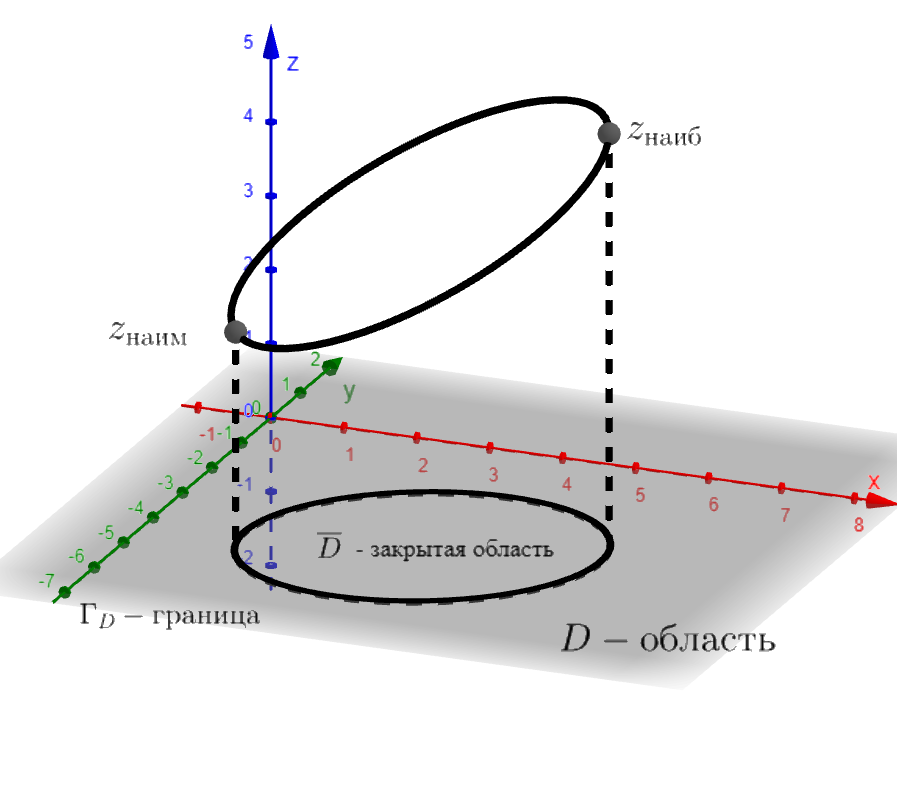
\includegraphics[height=90mm]{images/calculus_2024_02_28_3}

    Nota: Справедливы теоремы Вейерштрасса и Больцано-Коши для функции, непрерывной в заданной области

    $z = f(x, y)$ непрерывна на $\overline{D} = D \union \Gamma_D$, где $\overline{D}$ - закрытая область, $D$ - открытая область, $\Gamma_D$ - граница

    Th. W1 - $z = f(x, y)$ ограничена на $\overline{D}$

    Th. W2 - $\exists$ наибольшее и наименьшее $z \in \overline{D}$

    Th. B-C1 - на границе $\Gamma_D$ $z$ принимает значения разных знаков $\Longrightarrow \exists M \in \overline{D} : z(M) = 0$

    Th. B-C1 - $z(x, y)$ принимает все значения от $z_{\text{наим}}$ до $z_{\text{наиб}}$ \\[1\baselineskip]

    4.2 Производные функции двух переменных

    Путям $l_1, l_2$ соответствуют кривые $L_1, L_2$ на поверхности $z = f(x, y)$.

    Пользуясь геометрическим смыслом производной, заметим, что касательные к $L_1, L_2$ могут быть различными.


    Поэтому для определения производной выберем координатные направления $x = const$ и $y = const$

    $z = f(x = c, y)$

    $\displaystyle \frac{\partial z}{\partial y} \stackrel{def}{=} \lim_{\Delta y \to 0} \frac{\Delta_y z}{\Delta y}$,
    где $\Delta_y z = z(x, y + \Delta y) - z(x, y)$

    Определили частную производную $z$ по $y$

    Lab: Дать определение $\displaystyle \frac{\partial z}{\partial x}$

    Nota: $\Delta_y z = z(x, y + \Delta y) - z(x, y)$ и  $\Delta_y z$ называют частным приращением

    Def: Полное приращение $\Delta z \stackrel{def}{=} z(x + \Delta x, y + \Delta y) - z(x, y)$

    Nota! $\Delta z \neq \Delta_x z + \Delta_y z$

    Обозн.: $\displaystyle \frac{\partial z}{\partial x} = z^\prime_x = z_x$, $\displaystyle \frac{\partial z}{\partial y} = z^\prime_y = z_y$

    Как определить функцию, дифференцируемую в точке?

    По аналогии $\Delta z = A \Delta x + B \Delta y + \alpha \Delta x + \beta \Delta y$, где $A, B \in \Real$, $\alpha, \beta$ - б. м.

\end{document}
